\documentclass{article}
\usepackage[utf8]{inputenc}
\usepackage[T1]{fontenc}
\usepackage[rm={oldstyle=false}]{cfr-lm}
\usepackage[australian,american]{babel}

\usepackage[backend=biber,style=ieee,bibencoding=utf8,sorting=none,doi=false,isbn=false,url=false,date=short]{biblatex}
\usepackage{amssymb}
\usepackage{csquotes}
\usepackage[nolist]{acronym}
\usepackage{float}
\usepackage{todonotes}
\usepackage{pgfplots}
\usepackage{pgf}
\usepackage[binary-units]{siunitx}
\usepackage{pgfplotstable}
\usepackage{booktabs}
\usepackage{multirow}
\usepackage{lipsum}
\usepackage[hidelinks]{hyperref}
\usepackage{xspace}
\usetikzlibrary{patterns}

\usepgfplotslibrary{external, groupplots, units}
\tikzexternalize
\tikzsetexternalprefix{generated-figures/}
\pgfplotsset{compat=1.14}

\sisetup{
	round-mode          = places,
	round-precision     = 2,
}
\DeclareSIUnit\mbps{MB/s}

\pgfplotscreateplotcyclelist{my colors}{%
solid, color=black\\%
densely dotted, color=blue\\%
densely dashed, color=red\\%
}
\makeatother
%% Environment for comments: Set the boolean to false to produce a comment-free version.
\newboolean{showcomments}
\setboolean{showcomments}{true}
\ifthenelse{\boolean{showcomments}}
{ \newcommand{\mynote}[3]{
		\fbox{\bfseries\sffamily\scriptsize#1}
		{\small$\blacktriangleright$\textsf{\textit{\color{#3}{#2}}}$\blacktriangleleft$}}}
{ \newcommand{\mynote}[3]{}}
% One command per author:
\newcommand{\jt}[1]{\mynote{Jocelyn}{#1}{blue}}

\newcommand{\epto}{\textsc{EpTO}\xspace}
\newcommand{\jgroups}{\textsc{JGroups}\xspace}

\begin{document}

\section{Evaluation}
\subsection{Bandwidth}
\jt{\epto was run with $c=4$ to prevent any holes and a $\delta$ period of 100ms. Churn was run for 17minutes. 3min at the end with no churn, to see stabilization. Churn starts 30seconds after protocol}

\begin{figure}[h]
	\centering
	\begin{tikzpicture}
\usetikzlibrary{plotmarks}
\pgfplotsset{
	height=4cm,
	width=\linewidth / 2.6,
	every axis plot post/.append style={
		solid,
		very thin,
		mark=none
	},
	/pgfplots/area cycle list/.style={/pgfplots/cycle list={%
			{black,fill=black,mark=none},%
			{black,fill=white!25!black,mark=none},%
			{black,fill=white!50!black,mark=none},%
			{black,fill=white!75!black,mark=none},%
			{black,fill=white,mark=none},%
		}
	},
}
\begin{groupplot}[
ymajorgrids,
group style={
	group size=3 by 2,
	vertical sep=8mm,
	horizontal sep=4mm,
	xlabels at=edge bottom,
	ylabels at=edge left,
	yticklabels at=edge left,
},
stack plots=y,area style, enlarge x limits=false, 
ymin=0,
xmin=0,
ymax=4.5,
ytick={0,1,2,3,4},
yticklabels={0,1,2,3,4},
ylabel={Bandwidth $\left[\SI{}{\mbps}\right]$},
xlabel={Time $\left[\si{\minute}\right]$},
legend columns=5,
legend cell align=left,
legend style={at={(1.9,1.5)},anchor=north, font=\small, draw=none},]
\nextgroupplot[ymax=4,ytick={0,1,2,3,4},
yticklabels={0,1,2,3,4},]
\addplot table[x=time,y=EpTO-50-1sec-0.000000, col sep=comma]{\tableaverage} \closedcycle;
\addplot table[x=time,y=EpTO-50-1sec-0.250000, col sep=comma]{\tableaverage} \closedcycle;
\addplot table[x=time,y=EpTO-50-1sec-0.500000, col sep=comma]{\tableaverage} \closedcycle;
\addplot table[x=time,y=EpTO-50-1sec-0.750000, col sep=comma]{\tableaverage} \closedcycle;
\addplot table[x=time,y=EpTO-50-1sec-1.000000, col sep=comma]{\tableaverage} \closedcycle;
\legend{0, 0.25, 0.5, 0.75, 1}
%
\nextgroupplot[ymax=4,ytick={0,1,2,3,4},]
\addplot table[x=time,y=EpTO-50-2sec-0.000000, col sep=comma]{\tableaverage} \closedcycle;
\addplot table[x=time,y=EpTO-50-2sec-0.250000, col sep=comma]{\tableaverage} \closedcycle;
\addplot table[x=time,y=EpTO-50-2sec-0.500000, col sep=comma]{\tableaverage} \closedcycle;
\addplot table[x=time,y=EpTO-50-2sec-0.750000, col sep=comma]{\tableaverage} \closedcycle;
\addplot table[x=time,y=EpTO-50-2sec-1.000000, col sep=comma]{\tableaverage} \closedcycle;
%
\nextgroupplot[ymax=4,ytick={0,1,2,3,4},]
\addplot table[x=time,y=EpTO-100-1sec-0.000000, col sep=comma]{\tableaverage} \closedcycle;
\addplot table[x=time,y=EpTO-100-1sec-0.250000, col sep=comma]{\tableaverage} \closedcycle;
\addplot table[x=time,y=EpTO-100-1sec-0.500000, col sep=comma]{\tableaverage} \closedcycle;
\addplot table[x=time,y=EpTO-100-1sec-0.750000, col sep=comma]{\tableaverage} \closedcycle;
\addplot table[x=time,y=EpTO-100-1sec-1.000000, col sep=comma]{\tableaverage} \closedcycle;
%
\nextgroupplot[ymax=1.5,ytick={0,0.5,1,1.5},yticklabels={0,0.5,1,1.5},]
\addplot table[x=time,y=JGroups-50-1sec-0.000000, col sep=comma]{\tableaverage} \closedcycle;
\addplot table[x=time,y=JGroups-50-1sec-0.250000, col sep=comma]{\tableaverage} \closedcycle;
\addplot table[x=time,y=JGroups-50-1sec-0.500000, col sep=comma]{\tableaverage} \closedcycle;
\addplot table[x=time,y=JGroups-50-1sec-0.750000, col sep=comma]{\tableaverage} \closedcycle;
\addplot table[x=time,y=JGroups-50-1sec-1.000000, col sep=comma]{\tableaverage} \closedcycle;
%
\nextgroupplot[ymax=1.5,ytick={0,0.5,1,1.5},]
\addplot table[x=time,y=JGroups-50-2sec-0.000000, col sep=comma]{\tableaverage} \closedcycle;
\addplot table[x=time,y=JGroups-50-2sec-0.250000, col sep=comma]{\tableaverage} \closedcycle;
\addplot table[x=time,y=JGroups-50-2sec-0.500000, col sep=comma]{\tableaverage} \closedcycle;
\addplot table[x=time,y=JGroups-50-2sec-0.750000, col sep=comma]{\tableaverage} \closedcycle;
\addplot table[x=time,y=JGroups-50-2sec-1.000000, col sep=comma]{\tableaverage} \closedcycle;
%
\nextgroupplot[ymax=1.5,ytick={0,0.5,1,1.5},]
\addplot table[x=time,y=JGroups-100-1sec-0.000000, col sep=comma]{\tableaverage} \closedcycle;
\addplot table[x=time,y=JGroups-100-1sec-0.250000, col sep=comma]{\tableaverage} \closedcycle;
\addplot table[x=time,y=JGroups-100-1sec-0.500000, col sep=comma]{\tableaverage} \closedcycle;
\addplot table[x=time,y=JGroups-100-1sec-0.750000, col sep=comma]{\tableaverage} \closedcycle;
\addplot table[x=time,y=JGroups-100-1sec-1.000000, col sep=comma]{\tableaverage} \closedcycle;
\end{groupplot}
%
\node[anchor=south] at (group c1r1.north) {$(50,50)$};
\node[anchor=south] at (group c2r1.north) {$(50,100)$};
\node[anchor=south] at (group c3r1.north) {$(100,50)$};
\node[anchor=south, rotate=-90] at (group c3r1.east){\epto};
\node[anchor=south, rotate=-90] at (group c3r2.east){\jgroups};
\end{tikzpicture}
	\vspace{-2mm} 
	\caption{Throughput percentiles of a node during an experiment}
	\vspace{-2mm} 
	\label{fig:bandwidth}
\end{figure}
In \autoref{fig:bandwidth} we can see \epto has a worse baseline compared to \jgroups. It uses a median bandwidth of approximately \SI{1}{\mbps} for the smallest benchmark whereas \jgroups uses a median bandwidth of less than \SI{0.2}{\mbps}. However, in \jgroups most of the work is done solely by the coordinator. We can clearly see this as the 100th percentile is much higher than the rest and uses approximately \SI{.5}{\mbps}.

Comparing \epto and \jgroups in terms of bandwidth when we increase the number of events sent per second, we can see the bandwidth doubling in both cases.In lower peers scenario such as the ones presented in \autoref{fig:bandwidth} \jgroups is clearly at an advantage. Since \epto has a worse baseline we will reach the maximum bandwidth possible much quicker when increasing the event throughput.

Comparing \epto and \jgroups in terms of bandwidth when we increase the number of peers, \epto is performing better than \jgroups. Where \jgroups basically has to double the bandwidth usage of the coordinator, \epto only increases it by 50\% or less. \jt{logarithmic I think as was expected}. Thus in a scenario where we have many peers \epto will be more efficient than \jgroups at not reaching the maximum bandwidth.

\begin{figure}
	\centering
	\begin{tikzpicture}
\usetikzlibrary{plotmarks}
\pgfplotsset{
	height=4cm,
	width=\linewidth / 2,
	every axis plot post/.append style={
		solid,
		very thin,
		mark=none
	},
	/pgfplots/area cycle list/.style={/pgfplots/cycle list={%
			{black,fill=black,mark=none},%
			{black,fill=white!25!black,mark=none},%
			{black,fill=white!50!black,mark=none},%
			{black,fill=white!75!black,mark=none},%
			{black,fill=white,mark=none},%
		}
	},
}
\begin{groupplot}[
ymajorgrids,
group style={
	group size=2 by 3,
	vertical sep=8mm,
	horizontal sep=4mm,
	xlabels at=edge bottom,
	ylabels at=edge left,
	yticklabels at=edge left,
},
stack plots=y,area style, enlarge x limits=false, 
ymin=0,
xmin=0,
ylabel={Bandwidth $\left[\SI{}{\mbps}\right]$},
xlabel={Time $\left[\si{\minute}\right]$},
legend columns=5,
legend cell align=left,
legend style={at={(1.12,1.5)},anchor=north, font=\small, draw=none, fill=none},]
\nextgroupplot[ymax=4,ytick={0,1,2,3,4},
yticklabels={0,1,2,3,4},]
\addplot table[x=time,y=EpTO-suspend-0.000000, col sep=comma]{\tableaverage} \closedcycle;
\addplot table[x=time,y=EpTO-suspend-0.250000, col sep=comma]{\tableaverage} \closedcycle;
\addplot table[x=time,y=EpTO-suspend-0.500000, col sep=comma]{\tableaverage} \closedcycle;
\addplot table[x=time,y=EpTO-suspend-0.750000, col sep=comma]{\tableaverage} \closedcycle;
\addplot table[x=time,y=EpTO-suspend-1.000000, col sep=comma]{\tableaverage} \closedcycle;
\legend{0, 0.25, 0.5, 0.75, 1}
%
\nextgroupplot[ymax=4,ytick={0,1,2,3,4},]
\addplot table[x=time,y=EpTO-add-suspend-0.000000, col sep=comma]{\tableaverage} \closedcycle;
\addplot table[x=time,y=EpTO-add-suspend-0.250000, col sep=comma]{\tableaverage} \closedcycle;
\addplot table[x=time,y=EpTO-add-suspend-0.500000, col sep=comma]{\tableaverage} \closedcycle;
\addplot table[x=time,y=EpTO-add-suspend-0.750000, col sep=comma]{\tableaverage} \closedcycle;
\addplot table[x=time,y=EpTO-add-suspend-1.000000, col sep=comma]{\tableaverage} \closedcycle;
%
\nextgroupplot[ymax=20,ytick={0,5,10,15,20},
yticklabels={0,5,10,15,20},]
\addplot table[x=time,y=JGroups-suspend-coord-0.000000, col sep=comma]{\tableaverage} \closedcycle;
\addplot table[x=time,y=JGroups-suspend-coord-0.250000, col sep=comma]{\tableaverage} \closedcycle;
\addplot table[x=time,y=JGroups-suspend-coord-0.500000, col sep=comma]{\tableaverage} \closedcycle;
\addplot table[x=time,y=JGroups-suspend-coord-0.750000, col sep=comma]{\tableaverage} \closedcycle;
\addplot table[x=time,y=JGroups-suspend-coord-1.000000, col sep=comma]{\tableaverage} \closedcycle;
%
\nextgroupplot[ymax=20,ytick={0,5,10,15,20},]
\addplot table[x=time,y=JGroups-add-suspend-coord-0.000000, col sep=comma]{\tableaverage} \closedcycle;
\addplot table[x=time,y=JGroups-add-suspend-coord-0.250000, col sep=comma]{\tableaverage} \closedcycle;
\addplot table[x=time,y=JGroups-add-suspend-coord-0.500000, col sep=comma]{\tableaverage} \closedcycle;
\addplot table[x=time,y=JGroups-add-suspend-coord-0.750000, col sep=comma]{\tableaverage} \closedcycle;
\addplot table[x=time,y=JGroups-add-suspend-coord-1.000000, col sep=comma]{\tableaverage} \closedcycle;
%
\nextgroupplot[ymax=2,ytick={0,0.5,1,1.5,2},
yticklabels={0,0.5,1,1.5,2},]
\addplot table[x=time,y=JGroups-suspend-nocoord-0.000000, col sep=comma]{\tableaverage} \closedcycle;
\addplot table[x=time,y=JGroups-suspend-nocoord-0.250000, col sep=comma]{\tableaverage} \closedcycle;
\addplot table[x=time,y=JGroups-suspend-nocoord-0.500000, col sep=comma]{\tableaverage} \closedcycle;
\addplot table[x=time,y=JGroups-suspend-nocoord-0.750000, col sep=comma]{\tableaverage} \closedcycle;
\addplot table[x=time,y=JGroups-suspend-nocoord-1.000000, col sep=comma]{\tableaverage} \closedcycle;
%
\nextgroupplot[ymax=2,ytick={0,0.5,1,1.5,2},]
\addplot table[x=time,y=JGroups-add-suspend-nocoord-0.000000, col sep=comma]{\tableaverage} \closedcycle;
\addplot table[x=time,y=JGroups-add-suspend-nocoord-0.250000, col sep=comma]{\tableaverage} \closedcycle;
\addplot table[x=time,y=JGroups-add-suspend-nocoord-0.500000, col sep=comma]{\tableaverage} \closedcycle;
\addplot table[x=time,y=JGroups-add-suspend-nocoord-0.750000, col sep=comma]{\tableaverage} \closedcycle;
\addplot table[x=time,y=JGroups-add-suspend-nocoord-1.000000, col sep=comma]{\tableaverage} \closedcycle;
%
\end{groupplot}
\node[anchor=south] at (group c1r1.north) {1 kill};
\node[anchor=south] at (group c2r1.north) {1 \{kill,add\}/minute};
\node[anchor=south, rotate=-90] at (group c2r1.east){\epto};
\node[anchor=south, rotate=-90] at (group c2r2.east){\jgroups-coord};
\node[anchor=south, rotate=-90] at (group c2r3.east){\jgroups-nocoord};
\end{tikzpicture}
	\vspace{-2mm} 
	\caption{Throughput percentiles of a node during an experiment with churn}
	\vspace{-2mm} 
	\label{fig:bandwidth-churn}
\end{figure}

In \autoref{fig:bandwidth-churn} We analyze two different synthetic churns. In the first one we kill one node per minute. In the second one, we still kill one node per minute, but we immediately create a new one. For \jgroups we ran the benchmarks once without killing the coordinator and once killing it.

All tests were run using 100 peers and a global throughput of 50 events per second (100-1sec). \jt{I need to rephrase 50-1sec, 100-1sec etc. to be clearer}

We can see that the churn doesn't affect  \epto at all when there are only nodes leaving. We have small peaks when adding a node to \SI{3}{\mbps} or less. Probably due to running the PSS initialization method on top of having one more node spreading rumors in the system. This is confirmed at the end of the plot where \epto goes back to a normal Bandwidth after stabilization.

On the other hand, when killing the coordinator in \jgroups we can see a huge spike in bandwidth, going from \SI{1}{\mbps} to more than \SI{15}{\mbps}. This is due to how \jgroups operates when selecting a new coordinator.

Even when not killing the coordinator, \jgroups suffers from the churn. We can see that each time the view changes, it generates an almost 100\% increase in bandwidth usage. This is due to \jgroups having to update the view and propagate it to every peer.

\newpage

\subsection{Total Bytes sent/received}
\begin{figure}[h]
	\centering
	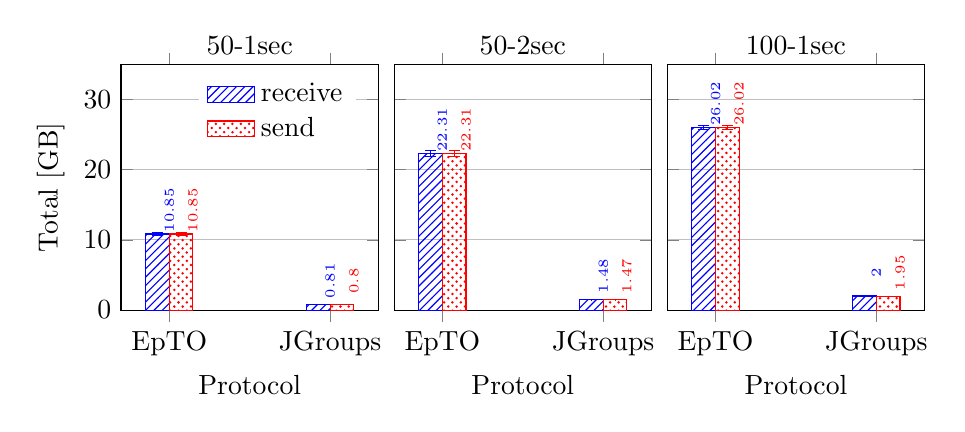
\begin{tikzpicture}
\usetikzlibrary{plotmarks}
\pgfplotsset{width=\linewidth, height=4.7cm}
\begin{groupplot}[
group style={
	group size=3 by 1,
	vertical sep=0pt,
	horizontal sep=2mm,
	xlabels at=edge bottom,
	ylabels at=edge left,
	xticklabels at=edge bottom,
	yticklabels at=edge left,
},
ymin=0,
ymax=35,
width=\linewidth / 2.5,
enlarge x limits=0.3,
ybar=0,
/pgf/bar width=3mm,
/pgfplots/area legend,
nodes near coords,
legend style={
	anchor=north west,
	at={(0.3,0.97)},
	cells={anchor=west},
	draw=none,
},
every node near coord/.append style={
	rotate=90,
	anchor=north,
	font=\tiny,
	xshift=3mm,
	yshift=0.3mm,
},
ymajorgrids,
xtick=data,
xlabel=Protocol,
ylabel={Total $\left[\si{\giga\byte}\right]$},
symbolic x coords={EpTO, JGroups},
]
\nextgroupplot
% 50-1sec
\addplot+[mark=none, pattern=north east lines,pattern color=blue, error bars/.cd,y dir=both, y explicit] coordinates {
	% Receive
	(EpTO, 10.8454953841) +- (0, 0.158556056880199)
	(JGroups, 0.8112389025) +- (0, 0.0275185471028981)
};
\addplot+[mark=none, pattern=crosshatch dots,pattern color=red, error bars/.cd,y dir=both, y explicit] coordinates {
	% Send
	(EpTO, 10.84508943053) +- (0, 0.158553532839913)
	(JGroups, 0.7979795057) +- (0, 0.0275124778152395)
};
\legend{receive, send}
\nextgroupplot
% 50-2sec
\addplot+[mark=none, pattern=north east lines,pattern color=blue, error bars/.cd,y dir=both, y explicit] coordinates {
	% Receive
	(EpTO, 22.3122950339) +- (0, 0.387040306037242)
	(JGroups, 1.481260734) +- (0, 0.0112693613185708)
};
\addplot+[mark=none, pattern=crosshatch dots,pattern color=red, error bars/.cd,y dir=both, y explicit] coordinates {
	% Send
	(EpTO, 22.3118855827) +- (0, 0.387040491969926)
	(JGroups, 1.4680794813) +- (0, 0.0112627440922006)
};
\nextgroupplot
% 100-1sec
\addplot+[mark=none, pattern=north east lines,pattern color=blue, error bars/.cd,y dir=both, y explicit] coordinates {
	% Receive
	(EpTO, 26.0194016553) +- (0, 0.2773178289900919968)
	(JGroups, 2.0044813206) +- (0, 0.0103933483299930001)
};
\addplot+[mark=none, pattern=crosshatch dots,pattern color=red, error bars/.cd,y dir=both, y explicit] coordinates {
	% Send
	(EpTO, 26.0161708501) +- (0, 0.277318407393540023)
	(JGroups, 1.9504773287) +- (0, 0.0104754176417391)
};
\end{groupplot}
%
\node[anchor=south] at (group c1r1.north) {50-1sec};
\node[anchor=south] at (group c2r1.north) {50-2sec};
\node[anchor=south] at (group c3r1.north) {100-1sec};
\end{tikzpicture}
	\vspace{-2mm} 
	\caption{Total bytes sent/received during an average experiment}
	\vspace{-2mm} 
	\label{fig:total-bandwidth}
\end{figure}
In \autoref{fig:total-bandwidth}, \epto has a worse baseline than \jgroups. This is expected as \epto sends $c*n*\log_2 n$ messages per events and \jgroups sends at least $n$ messages per event so we should have at least $c*\log_2 n$ more messages sent in \epto if \jgroups is perfect. Here we are well within this ratio.

\begin{figure}[h]
	\centering
	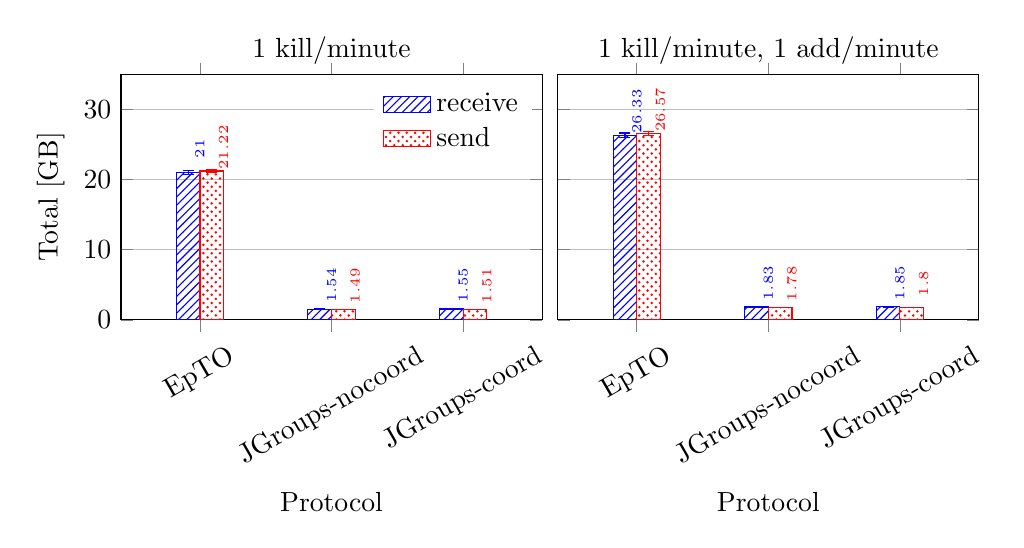
\begin{tikzpicture}
\usetikzlibrary{plotmarks}
\pgfplotsset{width=\linewidth, height=4.7cm}
\begin{groupplot}[
group style={
	group size=2 by 1,
	vertical sep=0pt,
	horizontal sep=2mm,
	xlabels at=edge bottom,
	ylabels at=edge left,
	xticklabels at=edge bottom,
	yticklabels at=edge left,
},
ymin=0,
ymax=35,
width=\linewidth / 1.75,
enlarge x limits=0.3,
ybar=0,
/pgf/bar width=3mm,
/pgfplots/area legend,
nodes near coords,
legend style={
	anchor=north west,
	at={(0.6,0.97)},
	cells={anchor=west},
	draw=none,
},
every node near coord/.append style={
	rotate=90,
	anchor=north,
	font=\tiny,
	xshift=3mm,
	yshift=0.3mm,
},
ymajorgrids,
xtick=data,
xlabel=Protocol,
xticklabel style={text height=1.5ex, rotate=30}, 
ylabel={Total $\left[\si{\giga\byte}\right]$},
symbolic x coords={EpTO, JGroups-nocoord, JGroups-coord},
]
\nextgroupplot
% 100-1sec 1kill/min
\addplot+[mark=none, pattern=north east lines,pattern color=blue, error bars/.cd,y dir=both, y explicit] coordinates {
	% Receive
	(EpTO, 21.001445292) +- (0, 0.248116313343146)
	(JGroups-nocoord, 1.5381357651) +- (0, 0.0115143286137117)
	(JGroups-coord, 1.5510862161) +- (0, 0.0181726968637206)
};
\addplot+[mark=none, pattern=crosshatch dots,pattern color=red, error bars/.cd,y dir=both, y explicit] coordinates {
	% Send
	(EpTO, 21.216776898) +- (0, 0.255744716454951)
	(JGroups-nocoord, 1.4935079775) +- (0, 0.0119366849923253)
	(JGroups-coord, 1.5064716889) +- (0, 0.0186384151121228)
};
\legend{receive, send}
\nextgroupplot
% 100-1sec 1kill, 1add/min
\addplot+[mark=none, pattern=north east lines,pattern color=blue, error bars/.cd,y dir=both, y explicit] coordinates {
	% Receive
	(EpTO, 26.325256447) +- (0, 0.320079175714576)
	(JGroups-nocoord, 1.8338254834) +- (0, 0.0187827622384514)
	(JGroups-coord, 1.8511940589) +- (0, 0.0183913437417294)
};
\addplot+[mark=none, pattern=crosshatch dots,pattern color=red, error bars/.cd,y dir=both, y explicit] coordinates {
	% Send
	(EpTO, 26.5733934455) +- (0, 0.320312180261336)
	(JGroups-nocoord, 1.7777051021) +- (0, 0.0190481557873808)
	(JGroups-coord, 1.7959073697) +- (0, 0.0189017779847593)
};
\end{groupplot}
%
\node[anchor=south] at (group c1r1.north) {1 kill/minute};
\node[anchor=south] at (group c2r1.north) {1 kill/minute, 1 add/minute};
\end{tikzpicture}
	\vspace{-2mm} 
	\caption{Total bytes sent/received during an average experiment with churn}
	\vspace{-2mm} 
	\label{fig:total-bandwidth-churn}
\end{figure}
In \autoref{fig:total-bandwidth-churn} we can see that \jgroups total bandwidth usage doesn't increase significantly compared to \epto with churn. An explanation for this phenomenon is that \jgroups takes more than a minute to find out the coordinator is effectively dead. During this time the bandwidth is practically not used. The big spike when the new coordinator is chosen compensates for this hole thus making the total bandwidth used appear as to not have changed.

The fact that killing the coordinator or not has no effect on the total bandwidth used tends to show the hypothesis to be correct.
\subsection{Local Times}
\label{sub:local-times}
\jt{Having a table for each percentile figure might be a good idea to put numbers for key percentiles (min,50th,max) for example}
\begin{figure}[h]
	\centering
	\input{figures/local-times.tex}
	\vspace{-2mm} 
	\caption{Local dissemination times}
	\vspace{-2mm}
	\label{fig:local-times} 
\end{figure}

\begin{figure}[h]
	\centering
	\input{figures/local-times-churn.tex}
	\vspace{-2mm} 
	\caption{Local dissemination times with churn}
	\vspace{-2mm} 
	\label{fig:local-times-churn} 
\end{figure}
In \autoref{fig:local-times}, \jgroups delivers all events quicker than \epto in all scenarios, even when churn is involved as is shown in \autoref{fig:local-times-churn}. However, \epto is not too far behind. The difference between \epto and \jgroups is likely to be even smaller when running them in a real WAN network due to the latency. \epto in our configuration has a $\delta$ period of \SI{100}{\milli\second} and is thus handicapped against \jgroups in a LAN environment, because it only increments the TTL of an event every \SI{100}{\milli\second}.
\newpage
\subsection{Global Times}
\begin{figure}[h]
	\centering
	\begin{tikzpicture}
\begin{groupplot}[
group style={
	group size=3 by 1,
	vertical sep=0pt,
	horizontal sep=6mm,
	xlabels at=edge bottom,
	ylabels at=edge left,
	xticklabels at=edge bottom,
	yticklabels at=edge left,
},
every axis plot/.append style={very thick},
width=\linewidth / 3,
height=5cm,
grid=major,
grid style={dashed,gray!30},
ymax=1.05,
ymin=0,
xmin=1185,
xmax=1202.5,
xlabel={Time $\left[\si{\second}\right]$},
x tick label style={/pgf/number format/fixed},
ytick={0,0.2,0.4,0.6,0.8,1},
yticklabels={0,0.2,0.4,0.6,0.8,1},
ylabel=Percentiles,
legend columns=3,
legend cell align=left,
legend style={at={(1.6,1.3)},anchor=north, font=\small, draw=none},
cycle list name=my colors,
]
\nextgroupplot
\addplot+[const plot, mark=none] table[x=EpTO-50-1sec-x, y=EpTO-50-1sec-y, col sep=comma] {\tableglobaltime};
\addplot+[const plot, mark=none] table[x=JGroups-50-1sec-x, y=JGroups-50-1sec-y, col sep=comma] {\tableglobaltime};
\legend{\epto, \jgroups}
%
\nextgroupplot
\addplot+[const plot, mark=none] table[x=EpTO-50-2sec-x, y=EpTO-50-2sec-y, col sep=comma] {\tableglobaltime};
\addplot+[const plot, mark=none] table[x=JGroups-50-2sec-x, y=JGroups-50-2sec-y, col sep=comma] {\tableglobaltime};
%
\nextgroupplot
\addplot+[const plot, mark=none] table[x=EpTO-100-1sec-x, y=EpTO-100-1sec-y, col sep=comma] {\tableglobaltime};
\addplot+[const plot, mark=none] table[x=JGroups-100-1sec-x, y=JGroups-100-1sec-y, col sep=comma] {\tableglobaltime};
\end{groupplot}
%
\node[anchor=south] at (group c1r1.north) {$(50,50)$};
\node[anchor=south] at (group c2r1.north) {$(50,100)$};
\node[anchor=south] at (group c3r1.north) {$(100,50)$};
\end{tikzpicture}
	\vspace{-2mm} 
	\caption{Global dissemination times}
	\vspace{-2mm}
	\label{fig:global-times}  
\end{figure}

\begin{figure}[h]
	\centering
	\input{figures/global-times-churn.tex}
	\vspace{-2mm} 
	\caption{Global dissemination times with churn}
	\vspace{-2mm} 
	\label{fig:global-times-churn} 
\end{figure}
We computed global times as well. They are represented in \autoref{fig:global-times} and \autoref{fig:global-times-churn}. These global times are of less interest than their local counterpart as the differences in clocks between hosts can skew this measurement.

Nonetheless, here too we can see that \epto is consistently slower than \jgroups for the same reason as stated in \autoref{sub:local-times}.
\newpage
\subsection{Local Dissemination stretch}
\begin{figure}[h]
	\centering
	\input{figures/local-delta.tex}
	\vspace{-2mm} 
	\caption{Local dissemination stretch}
	\vspace{-2mm}
	\label{fig:local-delta}  
\end{figure}
\jt{I wonder if we should split the plots (3 by 2) having a row for EpTO and a row for JGroups. This way we could show more for JGroups local dissemination stretch}In \autoref{fig:local-delta}, We can see the percentiles of the local dissemination stretch. The local dissemination stretch is the time measurement between the sending of an event by a peer and the delivery of this event locally.

\jgroups is usually much faster than \epto in a perfect environment. This is expected as the benchmarks involve a small number of nodes and are performed in a LAN environment with minmimal latency. The median dissemination stretch of \jgroups is around \SI{8}{\milli\second} where as the median dissemiantion stretch of \epto is around \SI{685}{\milli\second}. When increasing the number of peers, JGroups starts to have long delivery times

\begin{figure}[h]
	\centering
	\begin{tikzpicture}
\begin{groupplot}[
group style={
	group size=2 by 1,
	vertical sep=0pt,
	horizontal sep=6mm,
	xlabels at=edge bottom,
	ylabels at=edge left,
	xticklabels at=edge bottom,
	yticklabels at=edge left,
},
every axis plot/.append style={very thick},
height=5cm, width=\linewidth / 1.75,
grid=major,
grid style={dashed,gray!30},
ymax=1.05,
ymin=0,
xmax=25,
scaled x ticks = false,
x tick label style={/pgf/number format/fixed},
xlabel={Time $\left[\si{\second}\right]$},
ytick={0,0.2,0.4,0.6,0.8,1},
yticklabels={0,0.2,0.4,0.6,0.8,1},
ylabel=Percentiles,
legend columns=3,
legend cell align=left,
legend style={at={(1.1,1.3)},anchor=north, font=\small, draw=none, fill=none},
cycle list name=my colors,
]
\nextgroupplot
\addplot+[const plot, mark=none] table[x=EpTO-suspend-x, y=EpTO-suspend-y, col sep=comma] {\tablelocaldeltas};
\addplot+[const plot, mark=none] table[x=JGroups-suspend-coord-x, y=JGroups-suspend-coord-y, col sep=comma] {\tablelocaldeltas};
\addplot+[const plot, mark=nonee] table[x=JGroups-suspend-nocoord-x, y=JGroups-suspend-nocoord-y, col sep=comma] {\tablelocaldeltas};
\legend{\epto, \jgroups-coord, \jgroups-nocoord}
%
\nextgroupplot
\addplot+[const plot, mark=none] table[x=EpTO-add-suspend-x, y=EpTO-add-suspend-y, col sep=comma] {\tablelocaldeltas};
\addplot+[const plot, mark=none] table[x=JGroups-add-suspend-coord-x, y=JGroups-add-suspend-coord-y, col sep=comma] {\tablelocaldeltas};
\addplot+[const plot, mark=none] table[x=JGroups-add-suspend-nocoord-x, y=JGroups-add-suspend-nocoord-y, col sep=comma] {\tablelocaldeltas};
\end{groupplot}
%
\node[anchor=south] at (group c1r1.north) {1 kill/minute};
\node[anchor=south] at (group c2r1.north) {1 \{kill,add\}/minute};
\end{tikzpicture}
	\vspace{-2mm} 
	\caption{Local dissemination stretch with churn}
	\vspace{-2mm}
	\label{fig:local-delta-churn}   
\end{figure}
In \autoref{fig:local-delta-churn} We can see a completely different picture. When under churn, the 90th percentile of \jgroups is at \SI{447}{\milli\second} and the highest percentiles are at more than \SI{20}{\second} with the highest dissemination stretch being \SI{67.5}{\second}. This effect is due to the coordinator dying as we clearly see that it does not happen when we do not kill it.

The median is bigger at around \SI{11}{\milli\second}, whether we kill the coordinator or not. This shows that there are some degradation in \jgroups local dissemination stretch when under churn.

On the contrary, \epto performs very well under churn. The median stays really close at \SI{686}{\milli\second} with the 99.9th percentile being at \SI{1647}{\milli\second} compared to \SI{1366}{\milli\second} when no churn is happening.
\newpage
\subsection{Events sent}
\begin{figure}[h]
	\centering
	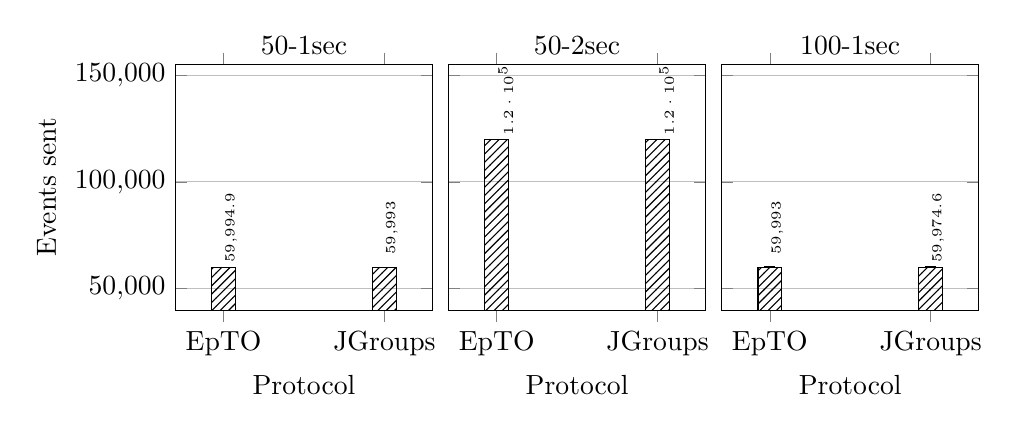
\begin{tikzpicture}
\usetikzlibrary{plotmarks}
\pgfplotsset{width=\linewidth, height=4.7cm}
\begin{groupplot}[
group style={
	group size=3 by 1,
	vertical sep=0pt,
	horizontal sep=2mm,
	xlabels at=edge bottom,
	ylabels at=edge left,
	xticklabels at=edge bottom,
	yticklabels at=edge left,
},
ymin=40000,
ymax=155000,
width=\linewidth / 2.5,
enlarge x limits=0.3,
ybar=0,
/pgf/bar width=3mm,
/pgfplots/area legend,
nodes near coords,
legend style={
	anchor=north west,
	at={(0.3,0.97)},
	cells={anchor=west},
	draw=none,
},
every node near coord/.append style={
	rotate=90,
	anchor=north,
	font=\tiny,
	xshift=5mm,
	yshift=1mm,
},
ymajorgrids,
xtick=data,
xlabel=Protocol,
ylabel={Events sent},
scaled ticks=false, tick label style={/pgf/number format/fixed},
symbolic x coords={EpTO, JGroups},
]
\nextgroupplot
% 50-1sec
\addplot[mark=none, pattern=north east lines, error bars/.cd,y dir=both, y explicit] coordinates {
	% Receive
	(EpTO, 59994.9) +- (0, 2.76686746259348)
	(JGroups, 59993) +- (0, 15.1217282962848)
};
%
\nextgroupplot
% 50-2sec
\addplot[mark=none, pattern=north east lines, error bars/.cd,y dir=both, y explicit] coordinates {
	% Receive
	(EpTO, 119908.5) +- (0, 8.04501225742594)
	(JGroups, 119924.7) +- (0, 5.69697775628018)
};
\nextgroupplot
% 100-1sec
\addplot[mark=none, pattern=north east lines, error bars/.cd,y dir=both, y explicit] coordinates {
	% Receive
	(EpTO, 59993) +- (0, 237.827201509368)
	(JGroups, 59974.6) +- (0, 216.060279654648)
};
\end{groupplot}
%
\node[anchor=south] at (group c1r1.north) {50-1sec};
\node[anchor=south] at (group c2r1.north) {50-2sec};
\node[anchor=south] at (group c3r1.north) {100-1sec};
\end{tikzpicture}
	\vspace{-2mm} 
	\caption{Total events sent per experiment on average}
	\vspace{-2mm}
	\label{fig:total-events}   
\end{figure}
In \autoref{fig:total-events} we can see that both \epto and \jgroups deliver the same amount of events. This is expected in a perfect environment.
\begin{figure}[h]
	\centering
	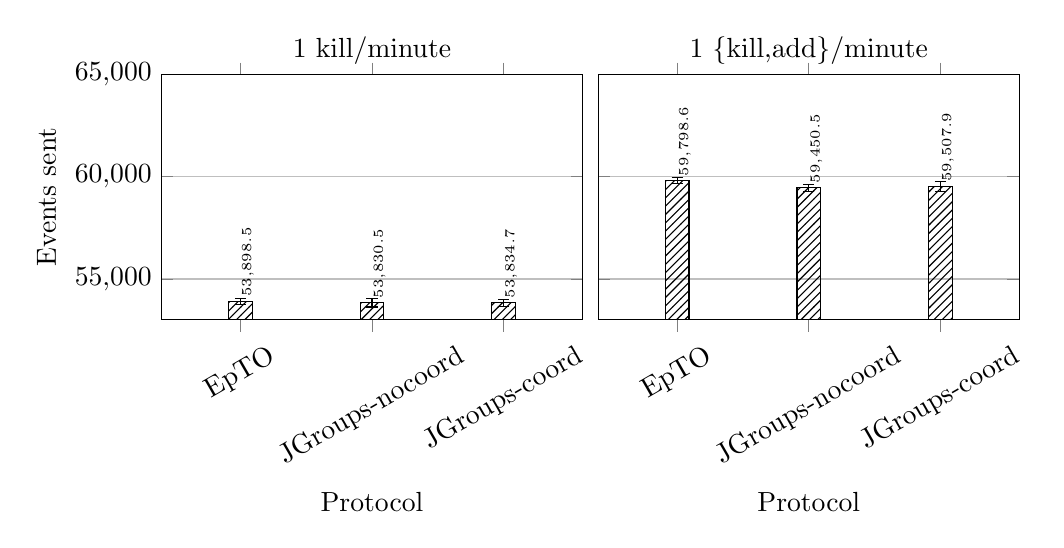
\begin{tikzpicture}
\pgfplotsset{width=\linewidth, height=4.7cm}
\begin{groupplot}[
group style={
	group size=2 by 1,
	vertical sep=0pt,
	horizontal sep=2mm,
	xlabels at=edge bottom,
	ylabels at=edge left,
	xticklabels at=edge bottom,
	yticklabels at=edge left,
},
ymin=53000,
ymax=65000,
width=\linewidth / 1.75,
enlarge x limits=0.3,
ybar=0,
/pgf/bar width=3mm,
/pgfplots/area legend,
nodes near coords,
legend style={
	anchor=north west,
	at={(0.6,0.97)},
	cells={anchor=west},
	draw=none,
},
every node near coord/.append style={
	rotate=90,
	anchor=north,
	font=\tiny,
	xshift=5mm,
	yshift=1mm,
},
ymajorgrids,
xtick=data,
xlabel=Protocol,
xticklabel style={text height=1.5ex, rotate=30}, 
scaled ticks=false, tick label style={/pgf/number format/fixed},
ylabel={Events sent},
symbolic x coords={EpTO, JGroups-nocoord, JGroups-coord},
]
\nextgroupplot
% 100-1sec 1kill/min
\addplot[mark=none, pattern=north east lines, error bars/.cd,y dir=both, y explicit] coordinates {
	% Receive
	(EpTO, 53898.5) +- (0, 133.952935350029)
	(JGroups-nocoord, 53830.5) +- (0, 200.355933278752)
	(JGroups-coord, 53834.7) +- (0, 175.463861426411)
};
%
\nextgroupplot
% 100-1sec 1kill, 1add/min
\addplot[mark=none, pattern=north east lines, error bars/.cd,y dir=both, y explicit] coordinates {
	% Receive
	(EpTO, 59798.6) +- (0, 140.107260498678)
	(JGroups-nocoord, 59450.5) +- (0, 175.171820412607)
	(JGroups-coord, 59507.9) +- (0, 240.914669079693)
};
\end{groupplot}
%
\node[anchor=south] at (group c1r1.north) {1 kill/minute};
\node[anchor=south] at (group c2r1.north) {1 \{kill,add\}/minute};
\end{tikzpicture}
	\vspace{-2mm} 
	\caption{Total events sent per experiment during churn on average}
	\vspace{-2mm}
	\label{fig:total-events-churn}  
\end{figure}

In \autoref{fig:total-events-churn} When only killing nodes, \epto and \jgroups again deliver the same amount of events.

However when killing and adding nodes \epto is clearly superior, delivering more than 2000 more events than \jgroups, even when \jgroups coordinator is not killed.

We are not sure why this is happening, but one hypothesis is that \jgroups peers take a longer time to join the cluster and thus start sending events later. Since the benchmarks start and stop at a given time, they send less events in total.



\end{document}
